\documentclass[12pt]{article}

\usepackage{fancyhdr}
\usepackage{amsthm}
\usepackage{amsmath}
\usepackage{graphicx}
\usepackage{amssymb}
\usepackage{esint}
\usepackage{subfigure}
\usepackage{color}
\usepackage{moreverb}
\usepackage{wrapfig}
\usepackage{csquotes}
\usepackage{url}
\graphicspath{ {images/} }
\textwidth 17cm \topmargin -1cm \oddsidemargin 0cm \textheight 21.5cm
\pagestyle{empty} \pagestyle{fancyplain}
\lhead[\fancyplain{}{}]{\fancyplain{}{{\sc Alexander Bauer}}}
\chead[\fancyplain{}{}]{\fancyplain{}{{\sc Home Work 01}}}
\rhead[\fancyplain{}{}]{\fancyplain{}{{\sc Computer Science 111}}}

\newcommand{\etal}{\textit{et al. }}

\begin{document}
\centerline{\Large\textbf{Free Fall With Drag, A Study of Numerical Solutions}}
\vspace{.3cm}


\section{Introduction}\label{sec::Intro}
Numerical solutions for ordinary differential equations (ODE) are methods used to find numerical approximations to the solutions of the ODE at a given point or at given points. I will be addressing the ODE: 
\begin{equation}
\left\{ % Note that we need to use \{ and not { to produce curly braces.
\begin{array}{cccc}
  \frac{dv}{dt} = g - \frac{c_d}{m}v^2 \\
  v(0) = 0
\end{array}
\right. % No curly brace on the right. We still need to put a dot.
\label{eq::curly}
\end{equation}

For this experiment time = 15s, g = 9.81 m/s^2, m = 75 kg, c_d = .25 kg/m. 

The exact solution of the ODE above is given by:

\begin{equation}
v(t) = \sqrt{\frac{gm}{c_d}}tanh(\sqrt{\frac{gc_d}{m}}t)
\end{equation}
I will be analyzing the accuracy of numeric solutions.

\section{Algorithm}
I analyzed the accuracy of three different methods of obtaining a numerical solution to the ODE mentioned in the introduction. 
We will go over the algorithms for
\begin{enumerate}
\item Euler's Method
\item Second Order Runge-Kutta Method
\item Fourth Order Runge-Kutta Method
\end{enumerate}
For all the following algorithms:
\begin{equation}
\left\{ % Note that we need to use \{ and not { to produce curly braces.
\begin{array}{cccc}
  y'(t) = f(t,y(t)) \\
  y_0 = y(t_0)
\end{array}
\right. % No curly brace on the right. We still need to put a dot.
\label{eq::curly}
\end{equation}
where y(t0) is the initial condition and is known.
\subsection{Using Euler's Method}\label{sec::using}
The Euler Method when used to calculate a numerical solution goes like this:
\begin{enumerate}
\item For a given step size, h, \begin{equation}
y(t+h) = y(t) + h \cdot f(t,y(t))
\end{equation}
\item Continue performing this calculation until \begin{equation}
t+h = t_f
\end{equation} where \begin{equation}
t_f
\end{equation} is the point at which you want to figure out the solution to the ODE 
\item \begin{equation}
y(t_f)
\end{equation} is the numerical solution to the ODE using Euler's Method

\end{enumerate}


\subsection{Second Order Runge-Kutta Method (RK2)}\label{sec::table}
The Second Order Runge-Kutta Method when used to calculate a numerical solution goes like this:
\begin{enumerate}
\item For a given step size, h, \begin{equation}
y(t+h) = y(t) + k_2
\end{equation}
\begin{equation}
k_1 = h \cdot f(t,y(t))
\end{equation}
\begin{equation}
k_2 = h \cdot f(t + h/2, y(t) + k_1/2)
\end{equation}
\item Continue performing this calculation until \begin{equation}
t+h = t_f
\end{equation} where \begin{equation}
t_f
\end{equation} is the point at which you want to figure out the solution to the ODE 
\item \begin{equation}
y(t_f)
\end{equation} is the numerical solution to the ODE using Euler's Method

\end{enumerate}

\subsection{Second Order Runge-Kutta Method (RK4)}\label{sec::table2}
The Fourth Order Runge-Kutta Method when used to calculate a numerical solution goes like this:
\begin{enumerate}
\item For a given step size, h, \begin{equation}
y(t+h) = y(t) + (k_1 + 2 \cdot k_2 + 2 \cdot k_3 + k_4)/6
\end{equation}
\begin{equation}
k_1 = h \cdot f(t,y(t))
\end{equation}
\begin{equation}
k_2 = h \cdot f(t + h/2, y(t) + k_1/2)
\end{equation}
\begin{equation}
k_3 = h \cdot f(t + h/2, y(t) + k_2/2)
\end{equation}
\begin{equation}
k_4 = h \cdot f(t + h, y(t) + k_3)
\end{equation}
\item Continue performing this calculation until \begin{equation}
t+h = t_f
\end{equation} where \begin{equation}
t_f
\end{equation} is the point at which you want to figure out the solution to the ODE 
\item \begin{equation}
y(t_f)
\end{equation} is the numerical solution to the ODE using Euler's Method

\end{enumerate}

\subsection{My Code}\label{sec::table3}
In my code I followed these algorithms exactly. I used a variable called \texttt{time step} in place of h, a variable called \texttt{velocity} instead of y(t), and a function called \texttt{acceleration} to solve for f(t, y(t)). In order to step through until the end time of 15s, I used a \texttt{for} loop that started at h and added h + t until it reached 15. Because of the way my for loop is set up, the end time must be divisible by the time step or the approximation will be off.

\section{Results}\label{sec::results}
In \texttt{MatLab}, my simulation code is invoked at the prompt by calling the function \texttt{FallingObjects}. The command
\newline\newline
\texttt{>> FallingObjects}
\newline\newline
will display 3 plots on the screen and four tables below the prompt. The plots consist of:
\begin{enumerate}
\item A plot of velocity vs time containing the exact velocity as a blue line and numerical approximations found using Euler's Method as open red circles
\item A plot of velocity vs time containing the exact velocity as a blue line and numerical approximations found using RK2 Method as open red circles
\item A plot of velocity vs time containing the exact velocity as a blue line and numerical approximations found using RK4 Method as open red circles
\end{enumerate}
The tables will consist of:
\begin{enumerate}
\item Table with five columns containing step size, approximations found with Euler's Method using those step sizes, the exact solution, the absolute error of each approximation, and the percent error of each approximation from left to right respectively.
\item Table with five columns containing step size, approximations found with RK2 Method using those step sizes, the exact solution, the absolute error of each approximation, and the percent error of each approximation from left to right respectively.
\item Table with five columns containing step size, approximations found with RK4 Method using those step sizes, the exact solution, the absolute error of each approximation, and the percent error of each approximation from left to right respectively.
\item Table with five columns containing step size, approximations found with Euler's Method using those step sizes, approximations found with RK2 using those step sizes, approximations found with RK4 using those step sizes, and the exact solution from left to right respectively.
\end{enumerate}

Here are the 3 plots:

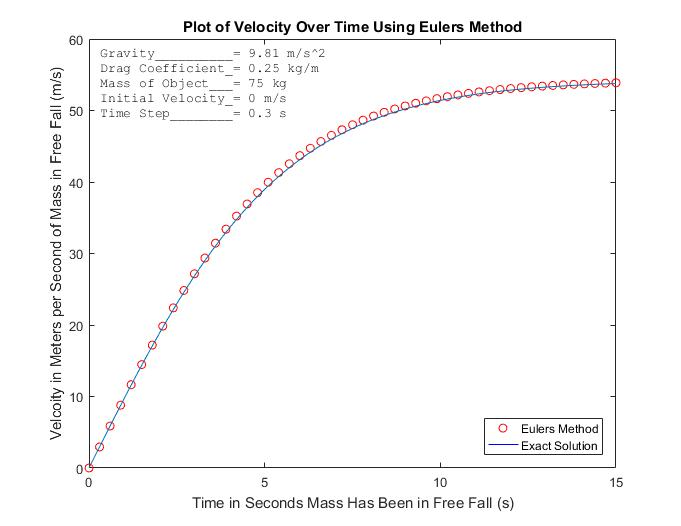
\includegraphics[scale=0.5]{EulersMethodPlot}

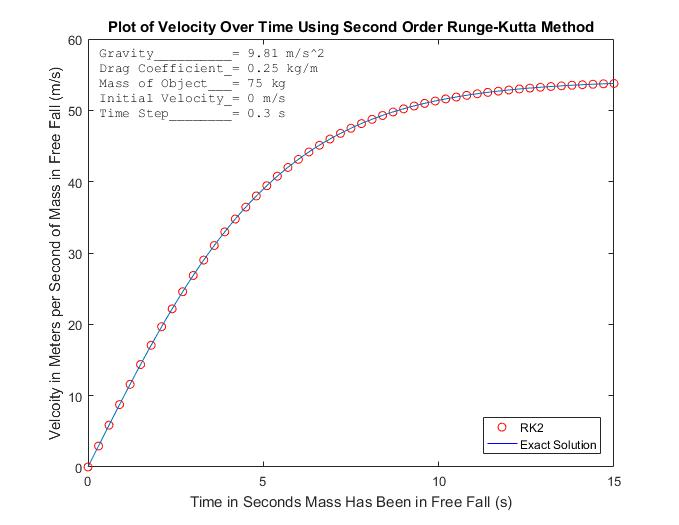
\includegraphics[scale=0.5]{RK2Plot}

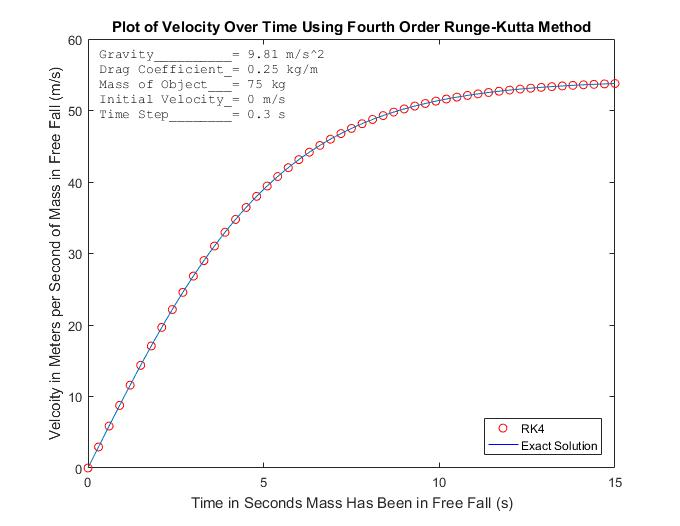
\includegraphics[scale=0.5]{RK4Plot}

Here are the 4 tables:

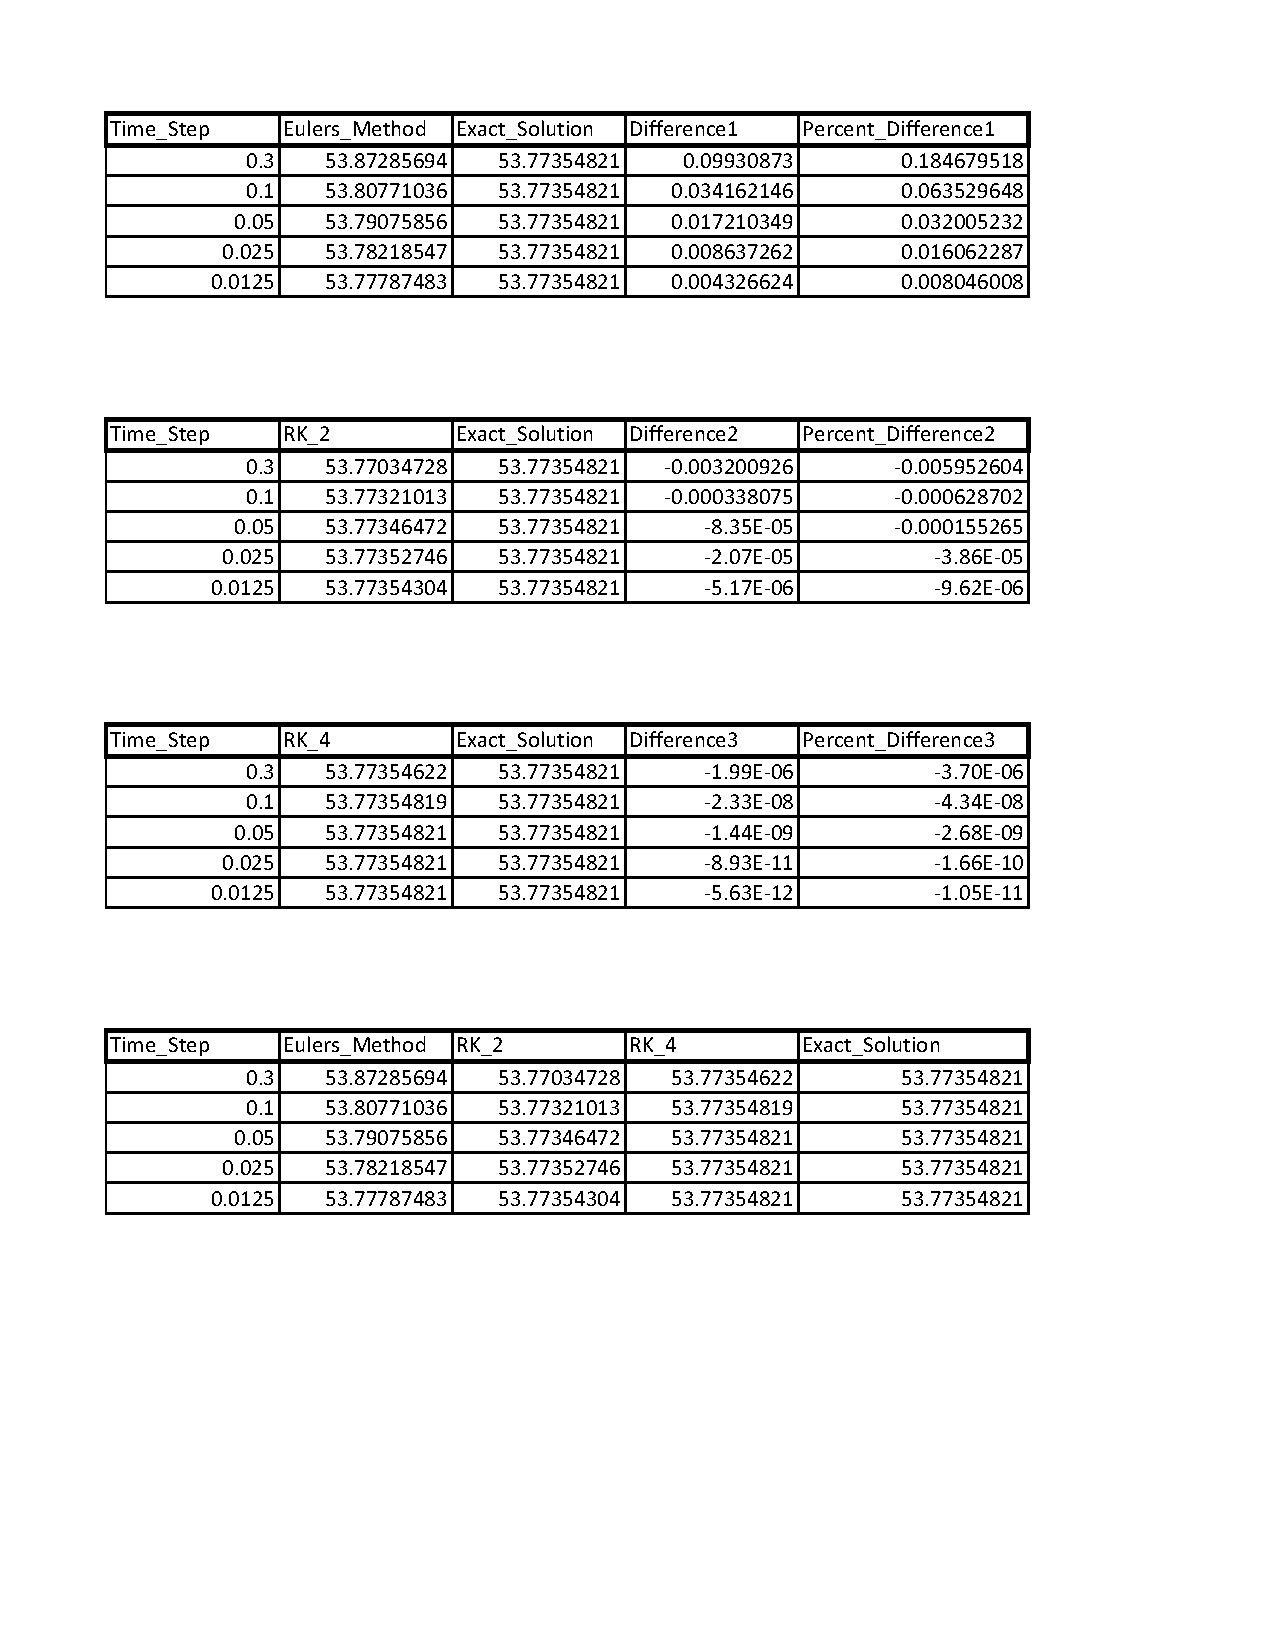
\includegraphics{Tables}

\section{Conclusion}\label{sec::conclusion}
Based on the plots you can tell that Euler's Method is less accurate than the RK2 and RK4 methods. However, it is hard to tell from the plots whether or not RK2 is more accurate than RK4 or vice-versa. Looking at the tables however, we can see that the absolute errors and percent differences are smaller for the RK4 method than for the RK2 method. So from the plots and tables we have determined the methods from most accurate to least accurate are as follows:
\begin{enumerate}
\item Fourth Order Runge-Kutta Method
\item Second Order Runge-Kutta Method
\item Euler's Method
\end{enumerate}
We can find the order of accuracy of each method by looking at the absolute errors. The order of accuracy is dependent on the method and can be found by looking at error and step size. A numerical solution is said to be nth order accurate if the error, E, is proportional to the step-size h to the nth power:
\begin{equation}
E(h) = Ch^n
\end{equation}
The corresponding big-O notation:
\begin{equation}
O(h^n)
\end{equation}
Looking at the tables, we see we have absolute error for the step sizes .1, .05, .025, and .0125. We can use these errors to determine the order of accuracy. For Eulers Method:
\begin{equation}
\left\{ % Note that we need to use \{ and not { to produce curly braces.
\begin{array}{cccc}
  E(.1) = 2 \cdot E(.05) = 4 \cdot E(.025) = 8 \cdot E(.0125) \\
  Ch_1^n = 2 \cdot C h_2^n \\
  h_1 = 2h_2 \\
  C2^nh_2^n = 2Ch_2^n \\
  2^n = 2 \\
  n = 1
\end{array}
\right. % No curly brace on the right. We still need to put a dot.
\label{eq::curly}
\end{equation}
The order of accuracy of Euler's Method is therefore 1.
For Second Order Runge-Kutta Method:
\begin{equation}
\left\{ % Note that we need to use \{ and not { to produce curly braces.
\begin{array}{cccc}
  E(.1) = 4 \cdot E(.05) = 16 \cdot E(.025) = 64 \cdot E(.0125) \\
  Ch_1^n = 4 \cdot Ch_2^n \\
  h_1 = 2h_2 \\
  C2^nh_2^n = 4Ch_2^n \\
  2^n = 4 \\
  n = 2
\end{array}
\right. % No curly brace on the right. We still need to put a dot.
\label{eq::curly}
\end{equation}
The order of accuracy of Second Order Runge-Kutta Method is therefore 2.
For Fourth Order Runge-Kutta Method:
\begin{equation}
\left\{ % Note that we need to use \{ and not { to produce curly braces.
\begin{array}{cccc}
  E(.1) = 16 \cdot E(.05) = 256 \cdot E(.025) = 4096 \cdot E(.0125) \\
  Ch_1^n = 16 \cdot Ch_2^n \\
  h_1 = 2h_2 \\
  C2^nh_2^n = 16Ch_2^n \\
  2^n = 16 \\
  n = 4
\end{array}
\right. % No curly brace on the right. We still need to put a dot.
\label{eq::curly}
\end{equation}
The order of accuracy of Fourth Order Runge-Kutta Method is therefore 4.

\clearpage
\appendix
\section{Implementation in MatLab}\label{sec::appendix}
The \texttt{MatLab} implementation with comments is given here:\newline\newline
\textbf{FallingObjects.m:}
\begin{verbatimtab}
% FallingObjects USES ALL THE OTHER FILES IN THIS DIRECTORY. IT PRODUCES THREE
% GRAPHS/PLOTS AND FOUR TABLES

g = 9.81;   %
c = .25;    % DEFINES GRAVITY, DRAG COEFFICIENT, AND MASS RESPECTIVELY, WHICH 
m = 75;     % WERE DEFINED IN THE HOMEWORK ASSIGNTMENT

EulersMethodPlot(.3,15,g,c,m); % CREATES THREE SEPERATE PLOTS OF THE EXACT
RK2Plot(.3,15,g,c,m);          % SOLUTION VS A NUMERICAL SOLUTION USING A
RK4Plot(.3,15,g,c,m);          % NUMERICAL METHOD

% THE REMAINDER OF THE PROGRAM DEALS WITH CREATING TABLES WHICH DEMONSTRATE THE
% ACCURACY OF EULERS METHOD, SECOND ORDER RUNGE-KUTTA METHOD, AND FOURTH ORDER
% RUNGE-KUTTA METHOD WHEN APPROXIMATING A NUMERICAL SOLUTION TO THE ORDINARY
% DIFFERENTIAL EQUATION GIVEN IN THE HOMEWORK

% CREATES A MATRIX OF EXACT SOLUTIONS FOR COMPARISON VALUE USEING Analytical
Exact_Solution = [Analytical(15,g,c,m);Analytical(15,g,c,m);...
                Analytical(15,g,c,m);Analytical(15,g,c,m);Analytical(15,g,c,m)];

% CREATES A MATRIX OF TIME STEPS
Time_Step = [.3; .1; .05; .025; .0125];

%%%%%%%%%%%%%%%%%%%%%%%%%%%%%%%%%%%%%%%%%%%%%%%%%%%%%%%%%%%%%%%%%%%%%%%%%%%%%%%%

% CREATES A MATRIX OF NUMERICAL SOLUTIONS USING THE STEP SIZES IN THE Time_Step
% MATRIX USING EULERS METHOD
Eulers_Method=[EulersMethod(.3,15,g,c,m);EulersMethod(.1,15,g,c,m);...
     EulersMethod(.05,15,g,c,m);EulersMethod(.025,15,g,c,m);...
     EulersMethod(.0125,15,g,c,m)];

% CREATES A MATRIX WITH THE DIFFERENCES BETWEEN THE APPROXIMATED SOLUTION FOUND
% USING EULERS METHOD AND THE EXACT SOLUTION FOR THE TIME STEPS IN THE 
% Time_Step MATRIX.
Difference1 = Eulers_Method - Exact_Solution;

% CREATES A MATRIX WITH THE PERCENT DIFFERENCE BETWEEN THE APPROXIMATED SOLUTION
% FOUND USING EULERS METHOD AND THE EXACT SOLUTION FOR THE TIME STEPS IN THE 
% Time_Step MATRIX.
Percent_Difference1=((Eulers_Method - Exact_Solution)/Analytical(15,g,c,m))*100;

%MAKE TABLE FOR EULERS METHOD
T1=table(Time_Step,Eulers_Method,Exact_Solution,Difference1,...
         Percent_Difference1);
disp(T1); % DISPLAY TABLE
writetable(T1,'T1.xls','sheet',1,'Range','B2:F7');
%%%%%%%%%%%%%%%%%%%%%%%%%%%%%%%%%%%%%%%%%%%%%%%%%%%%%%%%%%%%%%%%%%%%%%%%%%%%%%%%

% CREATES A MATRIX OF NUMERICAL SOLUTIONS USING THE STEP SIZES IN THE Time_Step
% MATRIX USING THE SECOND ORDER RUNGE-KUTTA METHOD
RK_2=[RK2(.3,15,g,c,m);RK2(.1,15,g,c,m);RK2(.05,15,g,c,m);RK2(.025,15,g,c,m);...
     RK2(.0125,15,g,c,m)];

% CREATES A MATRIX WITH THE DIFFERENCES BETWEEN THE APPROXIMATED SOLUTION FOUND
% USING SECOND ORDER RUNGE-KUTTA METHOD AND THE EXACT SOLUTION FOR THE TIME 
% STEPS IN THE Time_Step MATRIX.
Difference2 = RK_2 - Exact_Solution;
 
% CREATES A MATRIX WITH THE PERCENT DIFFERENCES BETWEEN THE APPROXIMATED 
% SOLUTION FOUND USING SECOND ORDER RUNGE-KUTTA METHOD AND THE EXACT SOLUTION 
% FOR THE TIME STEPS IN THE Time_Step MATRIX.
Percent_Difference2=((RK_2 - Exact_Solution)/Analytical(15,g,c,m))*100;

% MAKE TABLE FOR SECOND ORDER RUNGE-KUTTA METHOD (RK2)
T2=table(Time_Step,RK_2,Exact_Solution,Difference2,Percent_Difference2);
disp(T2); % DISPLAY TABLE
writetable(T2,'T2.xls','sheet',1,'Range','B2:F7');
%%%%%%%%%%%%%%%%%%%%%%%%%%%%%%%%%%%%%%%%%%%%%%%%%%%%%%%%%%%%%%%%%%%%%%%%%%%%%%%%

% CREATES A MATRIX OF NUMERICAL SOLUTIONS USING THE STEP SIZES IN THE Time_Step
% MATRIX USING THE FOURTH ORDER RUNGE-KUTTA METHOD
RK_4=[RK4(.3,15,g,c,m);RK4(.1,15,g,c,m);RK4(.05,15,g,c,m);RK4(.025,15,g,c,m);...
     RK4(.0125,15,g,c,m)];
 
% CREATES A MATRIX WITH THE DIFFERENCES BETWEEN THE APPROXIMATED SOLUTION FOUND
% USING FOURTH ORDER RUNGE-KUTTA METHOD AND THE EXACT SOLUTION FOR THE TIME 
% STEPS IN THE Time_Step MATRIX.
Difference3 = RK_4 - Exact_Solution;

% CREATES A MATRIX WITH THE PERCENT DIFFERENCES BETWEEN THE APPROXIMATED 
% SOLUTION FOUND USING FOURTH ORDER RUNGE-KUTTA METHOD AND THE EXACT SOLUTION 
% FOR THE TIME STEPS IN THE Time_Step MATRIX.
Percent_Difference3=((RK_4 - Exact_Solution)/Analytical(15,g,c,m))*100;

% MAKE TABLE FOR FOURTH ORDER RUNGE-KUTTA METHOD (RK4)
T3=table(Time_Step,RK_4,Exact_Solution,Difference3,Percent_Difference3);
disp(T3); % DISPLAY TABLE
writetable(T3,'T3.xls','sheet',1,'Range','B2:F7');
%%%%%%%%%%%%%%%%%%%%%%%%%%%%%%%%%%%%%%%%%%%%%%%%%%%%%%%%%%%%%%%%%%%%%%%%%%%%%%%%

% DISPLAYS A TABLE THAT SHOWS SOLUTIONS FOUND USING TIME STEPS IN Time_Step
% MATRIX FOR ALL NUMERICAL SOLUTION METHODS AND THE EXACT SOLUTION
T4 = table(Time_Step, Eulers_Method, RK_2, RK_4, Exact_Solution);
disp(T4); % DISPLAY TABLE
writetable(T4,'T4.xls','sheet',1,'Range','B2:F7');
\end{verbatimtab}
\textbf{acceleration.m:}
\begin{verbatimtab}
function dv_dt = acceleration(gravity, dragCoefficient, mass, velocity)

%acceleration SOLVES FOR THE ACCELERATION OF A GIVEN OBJECT AT A GIVEN TIME
%  THIS FUNCTION SOLVES THE ACCELERATION OF A MASS IN FREE FALL AFFECTED BY 
%   DRAG. THIS FUNCTION TAKES IN FOUR PARAMETERS: gravity, dragCoefficient, mass 
%   WHICH ARE ALL PARAMETERS THAT CAN BE PLAYED WITH FOR OBJECTS OF
%   DIFFERENT MASS WITH DIFFERENT DRAG COEFFICIENTS UNDER THE FORCE OF DIFFERENT
%   GRAVITY, AND velocity WHICH DEFINES THE VELOCITY OF THE OBJECT AT THE TIME
%   ACCELERATION NEEDS TO BE CALCULATED FOR

    g = gravity;            %
    c = dragCoefficient;    % VARIABLE DEFINITIONS THAT MAKE TYPING EASIER
    m = mass;               % 
    v = velocity;           %
    
    % CALCULATE ACCELERATION BASED ON PARAMETERS GIVEN
    dv_dt = g - (c/m) * v^2;
    % dv_dt NOW EQUALS THE ACCELERATION OF THE OBJECT AT VELCOITY velocity

end
\end{verbatimtab}
\textbf{Analytical.m:}
\begin{verbatimtab}
function exact_solution = Analytical(time, gravity, dragCoefficient, mass)

%Analytical SOLVES THE EXACT SOLUTION OF A GIVEN OBJECTS VELOCITY AT A GIVEN
%TIME
%  THIS FUNCTION SOLVES THE REAL VELOCITY OF A MASS IN FREE FALL AFFECTED BY 
%   DRAG. THIS FUNCTION TAKES IN FOUR PARAMETERS: time WHICH DEFINES THE TIME
%   AT WHICH VELOCITY SHOULD BE SOLVED FOR AND gravity, dragCoefficient, mass 
%   WHICH ARE ALL PARAMETERS THAT CAN BE PLAYED WITH FOR OBJECTS OF
%   DIFFERENT MASS WITH DIFFERENT DRAG COEFFICIENTS UNDER THE FORCE OF DIFFERENT
%   GRAVITY

    g = gravity;            %
    c = dragCoefficient;    % VARIABLE DEFINITIONS THAT MAKE TYPING EASIER
    m = mass;               % 
    t = time;               %
    
    % CALCULATE THE VELOCITY OF THE OBJACT AT TIME time SECONDS WHEN THE INITIAL
    % VELOCITY IS ZERO
    exact_solution = sqrt((g * m) / c) * tanh(sqrt((g * c) / m) * t);
    % exact_solution NOW EQUALS THE REAL VELOCITY OF THE OBJECT AT end_time
end
\end{verbatimtab}
\textbf{AnalyticalPlot.m:}
\begin{verbatimtab}
function exact_solution = AnalyticalPlot(time_step, end_time, gravity,...
                                         dragCoefficient, mass)
                                     
%AnalyticalPlot PLOTS THE EXACT SOLUTION OF A GIVEN OBJECTS VELOCITY AT A GIVEN
%TIME
%  THIS FUNCTION PLOTS THE REAL VELOCITY OF A MASS IN FREE FALL AFFECTED BY DRAG
%   THIS FUNCTION TAKES IN FIVE PARAMETERS: time_step WHICH DEFINES THE TIME
%   STEP BETWEEN EACH PLOT OF VELOCITY, end_time WHICH DEFINES HOW
%   LONG THE FREE FALL MOTION SHHOULD BE OBSERVED FOR, gravity, dragCoefficient,
%   and mass WHICH ARE ALL PARAMETERS THAT CAN BE PLAYED WITH FOR OBJECTS OF
%   DIFFERENT MASS WITH DIFFERENT DRAG COEFFICIENTS UNDER THE FORCE OF DIFFERENT
%   GRAVITY

    g = gravity;            %
    c = dragCoefficient;    % VARIABLE DEFINITIONS THAT MAKE TYPING EASIER
    m = mass;               % 
 
    % CALCULATE AND PLOT THE EXACT SOLUTION OF VELOCITY AT A 
    % GIVEN TIME FROM 0->end_time SECONDS
    t = (0:time_step:end_time);
    y = sqrt((g * m) / c) * tanh(sqrt((g * c) / m) * t);
    plot(t,y);
    
    exact_solution = sqrt((g * m) / c) * tanh(sqrt((g * c) / m) * end_time);
    % exact_solution NOW EQUALS THE REAL VELOCITY OF THE OBJECT AT end_time
end
\end{verbatimtab}
\textbf{EulersMethod.m:}
\begin{verbatimtab}
function velocity = EulersMethod(time_step, end_time, gravity,... 
                                 dragCoefficient, mass)
                             
%EulersMethod NUMERICALLY SOLVES THE VELOCITY OF AN OBJECT AFTER end_time
%SECONDS IN FREE FALL
%   THIS FUNCTION NUMERICALLY SOLVES THE VELOCITY OF A MASS IN FREE FALL 
%   AFFECTED BY DRAG USING EULERS METHOD. THIS FUNCTION TAKES IN FIVE PARAMETERS
%   : time_step WHICH DEFINES THE TIME STEP BETWEEN EACH ITERATION OF EULERS 
%   METHOD, end_time WHICH DEFINES HOW LONG THE FREE FALL MOTION SHHOULD BE 
%   OBSERVED FOR, AND gravity, dragCoefficient, and mass WHICH ARE ALL 
%   PARAMETERS THAT CAN BE PLAYED WITH FOR OBJECTS OF DIFFERENT MASS WITH 
%   DIFFERENT DRAG COEFFICIENTS UNDER THE FORCE OF DIFFERENT GRAVITY

    g = gravity;            %
    c = dragCoefficient;    % VARIABLE DEFINITIONS THAT MAKE TYPING EASIER
    m = mass;               % THE INITIAL TIME IS ALWAYS ZERO
    time = 0.0;             % THE INITIAL VELOCITY IS ALWAYS ZERO
    velocity = 0;           %
    
    % CALCULATE THE NUMERICAL APPROXIMATION OF VELOCITY AT A 
    % GIVEN TIME (endt_time) USING EULERS METHOD FOR ALL ITERATIONS OF 
    % EULERS METHOD. THE NUMBER OF ITERATIONS IS GIVEN BY end_time / time_step

    for time = time_step: time_step: end_time
        velocity = velocity + acceleration(g, c, m, velocity) * time_step;
    end
    % velocity NOW EQUALS THE NUMERICAL SOLUTION USING EULERS METHOD
end
\end{verbatimtab}
\textbf{EulersMethodPlot.m:}
\begin{verbatimtab}
function velocity = EulersMethodPlot(time_step, end_time, gravity,... 
                                 dragCoefficient, mass)
                             
%EulersMethodPlot PLOTS ITERATIONS OF EULERS METHOD WTIH THE GIVEN STEP SIZE
%UNTIL THE END TIME
%   THIS FUNCTION PLOTS THE VELOCITY OF A MASS IN FREE FALL AFFECTED BY DRAG.
%   THE PLOT USING EULERS METHOD TO NUMERICALLY SOLVE FOR VELOCITY IS SHOWN IN
%   RED CIRCLES WHILE THE EXACT SOLUTION IS SHOWN AS A BLUE LINE ON THE PLOT.
%   THIS FUNCTION TAKES IN FIVE PARAMETERS: time_step WHICH DEFINES THE TIME
%   STEP BETWEEN EACH ITERATION OF EULERS METHOD, end_time WHICH DEFINES HOW
%   LONG THE FREE FALL MOTION SHHOULD BE OBSERVED FOR, gravity, dragCoefficient,
%   and mass WHICH ARE ALL PARAMETERS THAT CAN BE PLAYED WITH FOR OBJECTS OF
%   DIFFERENT MASS WITH DIFFERENT DRAG COEFFICIENTS UNDER THE FORCE OF DIFFERENT
%   GRAVITY

    g = gravity;            %
    c = dragCoefficient;    % VARIABLE DEFINITIONS THAT MAKE TYPING EASIER
    m = mass;               % THE INITIAL TIME IS ALWAYS ZERO
    time = 0.0;             % THE INITIAL VELOCITY IS ALWAYS ZERO
    velocity = 0;           %

    % PLOT THE FIRST POINT OF EULERS METHOD AND CONFIGURE THE PLOT             %    
    figure
    plot(time, velocity,'or'); hold on;
    
    title('Plot of Velocity Over Time Using Eulers Method'); % PLOT TITLE
    xlabel('Time in Seconds Mass Has Been in Free Fall (s)');% AXIS LABELS    
    ylabel('Velcoity in Meters per Second of Mass in Free Fall (m/s)');
    %%%%%%%%%%%%%%%%%%%%%%%%%%%%%%%%%%%%%%%%%%%%%%%%%%%%%%%%%%%%%%%%%%%%%%%%%%%%
    str = {strjoin({'Gravity__________=',num2str(g),'m/s^2'}),strjoin(...      %
                   {'Drag Coefficient_=',num2str(c),'kg/m'}),strjoin(...       %
                   {'Mass of Object___=',num2str(m),'kg'}),strjoin(...         %
                   {'Initial Velocity_=',num2str(velocity),'m/s'}),strjoin(... %
                   {'Time Step________=',num2str(time_step),'s'})};            %
        % CONFIGURE INFORMATION DISPLAY THAT WILL GO ON THE PLOT %%%%%%%%%%%%%%%
    
    % CALCULATE AND PLOT THE NUMERICAL APPROXIMATION OF VELOCITY AT A 
    % GIVEN TIME USING EULERS METHOD FOR ALL ITERATIONS OF EULERS METHOD. 
    % THE NUMBER OF ITERATIONS IS GIVEN BY end_time / time_step
    for time = time_step: time_step: end_time
        velocity = velocity + acceleration(g,c,m,velocity) * time_step;
        plot(time, velocity,'or');hold on;
    end
    % velocity NOW EQUALS THE NUMERICAL SOLUTION USING EULERS METHOD
    
    % PLOT THE ACTUAL VELOCITY OF THE OBJECT OVER THE TIME INTERVAL 0->end_time
    AnalyticalPlot(.01, end_time, g, c, m);
    
    % THE REST OF THE CODE IS DEDICATED TO FORMATTING THE GRAPH    
    h = zeros(2, 1);                          %
    h(1) = plot(0,0,'or', 'visible', 'on');   % FORMAT LEGEND
    h(2) = plot(0,0,'-b', 'visible', 'on');   %
    legend(h, 'Eulers Method','Exact Solution','location','southeast');%
    
    t = text(end_time - (9.8*end_time)/10,velocity,str,'interpreter','none');
    t.FontName = 'FixedWidth'; % FORMAT ADDITIONAL INFORMATION TEXT
    

end
\end{verbatimtab}
\textbf{RK2.m:}
\begin{verbatimtab}
function velocity = RK2(time_step, end_time, gravity,... 
                        dragCoefficient, mass)
                    
%RK2 NUMERICALLY SOLVES THE VELOCITY OF AN OBJECT AFTER end_time
%SECONDS IN FREE FALL
%   THIS FUNCTION NUMERICALLY SOLVES THE VELOCITY OF A MASS IN FREE FALL 
%   AFFECTED BY DRAG USING A SECOND ORDER RUNGE-KUTTA APPROXIMATION (RK2). THIS
%   FUNCTION TAKES IN FIVE PARAMETERS: time_step WHICH DEFINES THE TIME STEP 
%   BETWEEN EACH ITERATION OF EULERS METHOD, end_time WHICH DEFINES HOW LONG THE
%   FREE FALL MOTION SHHOULD BE OBSERVED FOR, AND gravity, dragCoefficient, 
%   and mass WHICH ARE ALL PARAMETERS THAT CAN BE PLAYED WITH FOR OBJECTS OF 
%   DIFFERENT MASS WITH DIFFERENT DRAG COEFFICIENTS UNDER THE FORCE OF DIFFERENT
%   GRAVITY

    g = gravity;            %
    c = dragCoefficient;    % VARIABLE DEFINITIONS THAT MAKE TYPING EASIER
    m = mass;               % THE INITIAL TIME IS ALWAYS ZERO
    time = 0.0;             % THE INITIAL VELOCITY IS ALWAYS ZERO
    velocity = 0;           %
    
    % CALCULATE THE NUMERICAL APPROXIMATION OF VELOCITY AT A 
    % GIVEN TIME (endt_time) USING RK2 METHOD FOR ALL ITERATIONS OF 
    % RK2. THE NUMBER OF ITERATIONS IS GIVEN BY end_time / time_step
    for time = time_step: time_step: end_time
        k1 = time_step * acceleration(g,c,m,velocity);
        k2 = time_step * acceleration(g,c,m,velocity + k1 / 2);
        velocity = velocity + k2;
    end
    % velocity NOW EQUALS THE NUMERICAL SOLUTION USING THE SECOND ORDER
    % RUNGE-KUTTA METHOD
end
\end{verbatimtab}
\textbf{RK2Plot.m:}
\begin{verbatimtab}
function velocity = RK2Plot(time_step, end_time, gravity,... 
                        dragCoefficient, mass)
                    
%RK2Plot PLOTS ITERATIONS OF THE SECOND ORDER RUNGE-KUTTA (RK2) METHOD WTIH THE 
%GIVEN STEP SIZE UNTIL THE END TIME
%   THIS FUNCTION PLOTS THE VELOCITY OF A MASS IN FREE FALL AFFECTED BY DRAG.
%   THE PLOT USING THE RK2 METHOD TO NUMERICALLY SOLVE FOR VELOCITY IS SHOWN IN
%   RED CIRCLES WHILE THE EXACT SOLUTION IS SHOWN AS A BLUE LINE ON THE PLOT.
%   THIS FUNCTION TAKES IN FIVE PARAMETERS: time_step WHICH DEFINES THE TIME
%   STEP BETWEEN EACH ITERATION OF EULERS METHOD, end_time WHICH DEFINES HOW
%   LONG THE FREE FALL MOTION SHHOULD BE OBSERVED FOR, gravity, dragCoefficient,
%   and mass WHICH ARE ALL PARAMETERS THAT CAN BE PLAYED WITH FOR OBJECTS OF
%   DIFFERENT MASS WITH DIFFERENT DRAG COEFFICIENTS UNDER THE FORCE OF DIFFERENT
%   GRAVITY

    g = gravity;            %
    c = dragCoefficient;    % VARIABLE DEFINITIONS THAT MAKE TYPING EASIER
    m = mass;               % THE INITIAL TIME IS ALWAYS ZERO
    time = 0.0;             % THE INITIAL VELOCITY IS ALWAYS ZERO
    velocity = 0;           %

    % PLOT THE FIRST POINT OF RK2 AND CONFIGURE THE PLOT             %    
    figure
    plot(time, velocity,'or'); hold on;
    
    title('Plot of Velocity Over Time Using Second Order Runge-Kutta Method');
    xlabel('Time in Seconds Mass Has Been in Free Fall (s)');% AXIS LABELS    
    ylabel('Velcoity in Meters per Second of Mass in Free Fall (m/s)');
    %%%%%%%%%%%%%%%%%%%%%%%%%%%%%%%%%%%%%%%%%%%%%%%%%%%%%%%%%%%%%%%%%%%%%%%%%%%%
    str = {strjoin({'Gravity__________=',num2str(g),'m/s^2'}),strjoin(...      %
                   {'Drag Coefficient_=',num2str(c),'kg/m'}),strjoin(...       %
                   {'Mass of Object___=',num2str(m),'kg'}),strjoin(...         %
                   {'Initial Velocity_=',num2str(velocity),'m/s'}),strjoin(... %
                   {'Time Step________=',num2str(time_step),'s'})};            %
        % CONFIGURE INFORMATION DISPLAY THAT WILL GO ON THE PLOT %%%%%%%%%%%%%%%
    
    % CALCULATE AND PLOT THE NUMERICAL APPROXIMATION OF VELOCITY AT A 
    % GIVEN TIME USING RK2 METHOD FOR ALL ITERATIONS OF RK2. THE NUMBER OF
    % ITERATIONS IS GIVEN BY end_time / time_step
    for time = time_step: time_step: end_time
        k1 = time_step * acceleration(g,c,m,velocity);
        k2 = time_step * acceleration(g,c,m,velocity + k1 / 2);
        velocity = velocity + k2;
        plot(time, velocity,'or');hold on;
    end
    % velocity NOW EQUALS THE NUMERICAL SOLUTION USING THE SECOND ORDER
    % RUNGE-KUTTA METHOD

    % PLOT THE ACTUAL VELOCITY OF THE OBJECT OVER THE TIME INTERVAL 0->end_time
    AnalyticalPlot(.01, end_time, g, c, m);
    
    % THE REST OF THE CODE IS DEDICATED TO FORMATTING THE GRAPH    
    h = zeros(2, 1);                          %
    h(1) = plot(0,0,'or', 'visible', 'on');   % FORMAT LEGEND
    h(2) = plot(0,0,'-b', 'visible', 'on');   %    
    legend(h, 'RK2','Exact Solution','location','southeast');
    
    t = text(end_time - (9.8*end_time)/10,velocity,str,'interpreter','none');
    t.FontName = 'FixedWidth'; % FORMAT ADDITIONAL INFORMATION TEXT

end
\end{verbatimtab}
\textbf{RK4.m:}
\begin{verbatimtab}
function velocity = RK4(time_step, end_time, gravity,... 
                        dragCoefficient, mass)
                    
%RK4 NUMERICALLY SOLVES THE VELOCITY OF AN OBJECT AFTER end_time
%SECONDS IN FREE FALL
%   THIS FUNCTION NUMERICALLY SOLVES THE VELOCITY OF A MASS IN FREE FALL 
%   AFFECTED BY DRAG USING A FOURTH ORDER RUNGE-KUTTA APPROXIMATION (RK4). THIS
%   FUNCTION TAKES IN FIVE PARAMETERS: time_step WHICH DEFINES THE TIME STEP 
%   BETWEEN EACH ITERATION OF EULERS METHOD, end_time WHICH DEFINES HOW LONG THE
%   FREE FALL MOTION SHHOULD BE OBSERVED FOR, AND gravity, dragCoefficient, 
%   and mass WHICH ARE ALL PARAMETERS THAT CAN BE PLAYED WITH FOR OBJECTS OF 
%   DIFFERENT MASS WITH DIFFERENT DRAG COEFFICIENTS UNDER THE FORCE OF DIFFERENT
%   GRAVITY

    g = gravity;            %
    c = dragCoefficient;    % VARIABLE DEFINITIONS THAT MAKE TYPING EASIER
    m = mass;               % THE INITIAL TIME IS ALWAYS ZERO
    time = 0.0;             % THE INITIAL VELOCITY IS ALWAYS ZERO
    velocity = 0;           %
    
    % CALCULATE THE NUMERICAL APPROXIMATION OF VELOCITY AT A 
    % GIVEN TIME (endt_time) USING RK4 METHOD FOR ALL ITERATIONS OF 
    % RK4. THE NUMBER OF ITERATIONS IS GIVEN BY end_time / time_step
    for time = time_step: time_step: end_time
        k1 = time_step * acceleration(g,c,m,velocity);
        k2 = time_step * acceleration(g,c,m,velocity + k1 / 2);
        k3 = time_step * acceleration(g,c,m,velocity + k2 / 2);
        k4 = time_step * acceleration(g,c,m,velocity + k3);
        velocity = velocity + (k1 + 2*k2 + 2*k3 + k4) / 6;
    end
    % velocity NOW EQUALS THE NUMERICAL SOLUTION USING THE FOURTH ORDER
    % RUNGE-KUTTA METHOD
end
\end{verbatimtab}
\textbf{RK4Plot.m:}
\begin{verbatimtab}
function velocity = RK4Plot(time_step, end_time, gravity,... 
                        dragCoefficient, mass)
                    
%RK4Plot PLOTS ITERATIONS OF THE FOURTH ORDER RUNGE-KUTTA (RK2) METHOD WTIH THE 
%GIVEN STEP SIZE UNTIL THE END TIME
%   THIS FUNCTION PLOTS THE VELOCITY OF A MASS IN FREE FALL AFFECTED BY DRAG.
%   THE PLOT USING THE RK4 METHOD TO NUMERICALLY SOLVE FOR VELOCITY IS SHOWN IN
%   RED CIRCLES WHILE THE EXACT SOLUTION IS SHOWN AS A BLUE LINE ON THE PLOT.
%   THIS FUNCTION TAKES IN FIVE PARAMETERS: time_step WHICH DEFINES THE TIME
%   STEP BETWEEN EACH ITERATION OF EULERS METHOD, end_time WHICH DEFINES HOW
%   LONG THE FREE FALL MOTION SHHOULD BE OBSERVED FOR, gravity, dragCoefficient,
%   and mass WHICH ARE ALL PARAMETERS THAT CAN BE PLAYED WITH FOR OBJECTS OF
%   DIFFERENT MASS WITH DIFFERENT DRAG COEFFICIENTS UNDER THE FORCE OF DIFFERENT
%   GRAVITY

    g = gravity;            %
    c = dragCoefficient;    % VARIABLE DEFINITIONS THAT MAKE TYPING EASIER
    m = mass;               % THE INITIAL TIME IS ALWAYS ZERO
    time = 0.0;             % THE INITIAL VELOCITY IS ALWAYS ZERO
    velocity = 0;           %

    % PLOT THE FIRST POINT OF RK4 AND CONFIGURE THE PLOT             %    
    figure
    plot(time, velocity,'or'); hold on;
    
    title('Plot of Velocity Over Time Using Second Order Runge-Kutta Method');
    xlabel('Time in Seconds Mass Has Been in Free Fall (s)');% AXIS LABELS    
    ylabel('Velcoity in Meters per Second of Mass in Free Fall (m/s)');
    %%%%%%%%%%%%%%%%%%%%%%%%%%%%%%%%%%%%%%%%%%%%%%%%%%%%%%%%%%%%%%%%%%%%%%%%%%%%
    str = {strjoin({'Gravity__________=',num2str(g),'m/s^2'}),strjoin(...      %
                   {'Drag Coefficient_=',num2str(c),'kg/m'}),strjoin(...       %
                   {'Mass of Object___=',num2str(m),'kg'}),strjoin(...         %
                   {'Initial Velocity_=',num2str(velocity),'m/s'}),strjoin(... %
                   {'Time Step________=',num2str(time_step),'s'})};            %
        % CONFIGURE INFORMATION DISPLAY THAT WILL GO ON THE PLOT %%%%%%%%%%%%%%%
    
    % CALCULATE AND PLOT THE NUMERICAL APPROXIMATION OF VELOCITY AT A 
    % GIVEN TIME USING RK4 METHOD FOR ALL ITERATIONS OF RK4. THE NUMBER OF
    % ITERATIONS IS GIVEN BY end_time / time_step
    for time = time_step: time_step: end_time
        k1 = time_step * acceleration(g,c,m,velocity);
        k2 = time_step * acceleration(g,c,m,velocity + k1 / 2);
        k3 = time_step * acceleration(g,c,m,velocity + k2 / 2);
        k4 = time_step * acceleration(g,c,m,velocity + k3);
        velocity = velocity + (k1 + 2*k2 + 2*k3 + k4) / 6;
        plot(time, velocity,'or');hold on;
    end
    % velocity NOW EQUALS THE NUMERICAL SOLUTION USING THE FOURTH ORDER
    % RUNGE-KUTTA METHOD
    
    % PLOT THE ACTUAL VELOCITY OF THE OBJECT OVER THE TIME INTERVAL 0->end_time    
    AnalyticalPlot(.01, end_time, g, c, m);
    
    % THE REST OF THE CODE IS DEDICATED TO FORMATTING THE GRAPH    
    h = zeros(2, 1);                          %
    h(1) = plot(0,0,'or', 'visible', 'on');   % FORMAT LEGEND
    h(2) = plot(0,0,'-b', 'visible', 'on');   %    
    legend(h, 'RK4','Exact Solution','location','southeast');
    
    t = text(end_time - (9.8*end_time)/10,velocity,str,'interpreter','none');
    t.FontName = 'FixedWidth'; % FORMAT ADDITIONAL INFORMATION TEXT

    
end
\end{verbatimtab}
\newpage
\clearpage
\bibliographystyle{plain}
\bibliography{bibfile}
\setcounter{page}{1} \pagestyle{empty}


%%%%%%%%%%%

\end{document}
